\chapter{Introduction}

\chapter{Nucleon Internal Structure Phenomenology}

The topic of this paper, simply put, is the exploration of the momentum structure of 
the \emph{nucleon}, a particle that makes up an atom's nucleus which can be either a
proton (\emph{p}) or a neutron (\emph{n}). By momentum structure, I refer to the
fractional momentum distributions carried by the nucleon's constituent particles,
quarks and gluons.

While a complete review of the history and physics behind nucleon structure and its
investigative probes is beyond the scope of this paper, a brief overview of deep-inelastic
scattering and Drell-Yan will help in understanding concepts and terminology relevant to this and later chapters.

\section{Introduction}

The first indication that the proton may have some internal structure was in a
1933 experiment by Estermann \emph{et al.} measuring the magnetic moment of the proton 
\cite{Estermann:169E}. Since the proton was thought to be a point-like Dirac particle, it's 
magnetic moment ($\mu_p$) was expected to be $\mu_p = \frac{e}{2 m_p} = 1 n.m.$, or one \emph{nuclear magneton}. The experiment resulted in a value of 2.5 n.m., leading many
to reconsider the notion that the proton is indeed point-like.

Around the same time, Hideku Yukawa is credited for establishing the first theory
of a \emph{strong force}, a force binding together nucleons in a nuclei against the sizable
\emph{Coulomb} repulsion of protons \cite{}.
The force was theorized to be mediated by the exchange of particles called \emph{mesons}, 
and its range was limited to nuclei-scale distances, seeing as it's not observed at larger distances. Based upon the size of the nucleus, Yukawa estimated the mass of the intermediating particles to be approximately $2 \times 10^2 m_e \approx 100 MeV$, where $m_e$ is the electron mass. 
The following year, Anderson et al. discovered the muon ($\mu$) at around this mass \cite{},
which confused many, as it did not seem to partake in strong interactions. Eventually, by 1947,
the meson theory was validated by the discovery of the \emph{pion} by Powell 
\emph{et al.} \cite{}, and Yukawa was awarded a Nobel Prize for his theory in 1949.

While the 

The study of nucleon structure has come a long way, and at present, the proton 
is described as a composite particle consisting of three point-like \emph{valence quarks}
interacting with each other through exchange of gluons.






\section{\emph{ep} Scattering}

Nucleon structure is still today one of the great frontiers of nuclear physics.  The primary tool used to probe the parton distribution has been Deep Inelastic Scattering (DIS), which is the scattering of a charged lepton off of a nucleus by the exchange of a virtual photon.  As the energy of the exchanged photon increases, the scattering becomes inelastic and is able to resolve the partonic substructure of hadrons.

\section{The Drell-Yan Process}

\begin{figure}[h]
	\centering
	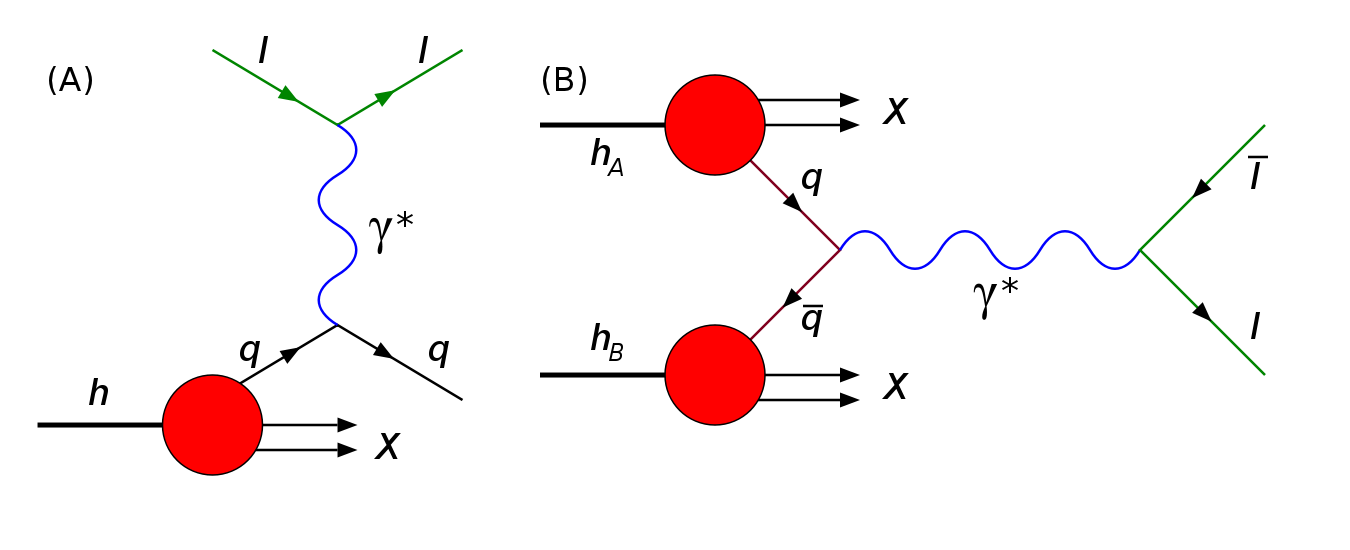
\includegraphics[width=4.50in]{figures/DIS-DY}
	\caption{(A) Deep inelastic scattering (DIS) is a $t$-channel interaction which uses the emission of a virtual photon to probe the target hadron. (B) The similar Drell-Yan (DY) process, using the $s$ channel version of the DIS interaction, via annihilation of a beam quark with an anti-quark from the target hadron.}
	\label{fig:dis-dy}
\end{figure}

As useful as this has been, DIS is only sensitive to momentum and charge of the partonic structure.

In 1970, S. Drell and T.M. Yan were the first to study the process in which high-mass lepton production occurs as a result of inelastic hadron-hadron collisions \cite{Drell:1970wh}.  This so-called "Drell-Yan" (DY) process is identified to be the result of a quark-antiquark annihilation into a virtual photon which then decays into a lepton pair. 

This process, as you see in Figure \ref{fig:dis-dy}, is the \emph{s}-channel counterpart to DIS's \emph{t}-channel process.  Similarly Drell-Yan can give a complementary view of the nucleon's parton distribution. The differential cross section that we will be using is in terms of the fractional momentum variables, $x_1$ and $x_2$, which represent the fraction of the respective hadron's momentum carried by the beam quark and target anti-quark, respectively.

To begin, we start with the annihilation cross section for $e^+e^- \rightarrow \mu^+\mu^-$ and simply add a color factor of $\frac{1}{3}$ since only like flavor-antiflavor quarks will annihilate, and use the charge $e_i^2$ for quark flavor $i$ \cite{duan-2007-50}. Other variables referred to in Eq \ref{eq:DY-cross1} and \ref{eq:DY-cross2} and more are defined in Table \ref{tab:var}.

\begin{equation}
\frac{d\hat{\sigma}}{dM} = \frac{8 \pi \alpha^2}{9M}e_i^2\delta(\hat{s} - M^2)
\label{eq:DY-cross1}
\end{equation}

The hadronic Drell-Yan differential cross section can be obtained from this by the convolution of the above cross section with the quark distributions in the beam and target.

\begin{equation}
\frac{d^2\sigma^{DY}}{dx_1x_2}=\frac{8\pi\alpha^2}{9sx_1x_2 K(x_1,x_2)}
\sum_{i}e_i^2[q_i^b(x_1)\bar{q}_i^t(x_2)+
\bar{q}_i^b(x_1)q_i^t(x_2)]
\label{eq:DY-cross2}
\end{equation}

\begin{table}[h]
	\centering
	\begin{tabular}{ccl}
		Variable&Description\\ \hline \hline
		$\alpha$ & The fine structure constant \\
		$K(x_1,x_2)$ & High-order QCD correction term \\ \hline
		$\sqrt{s}$ & The center of mass energy of the hadronic collision \\
		$\sqrt{\hat{s}}$ & The center of mass energy of the $q\bar{q}$ collision \\
		$Q^{2}$ & The four-momentum of the intermediate time-like photon, squared \\ 
		$q_i^{t/b}(x)$ & The quark number density in the nucleon of the target/beam \\ \hline \hline
	\end{tabular}
	\caption{Kinematic variables relevant to the Drell-Yan process .}
	\label{tab:var}
\end{table}


In addition to the leading-order DY term, there are high-order QCD corrections to consider. These have been studied and accounted for up to $O(\alpha_s)$ and $O(\alpha_s^2)$. These include contributions from high-order $q\bar{q}$ annihilation $(q \bar{q} \rightarrow \gamma * + g)$ and gluon Compton scattering $(q + g \rightarrow \gamma * + q)$ as seen in Figure \ref{fig:nlo-dy} \cite{duan-2007-50}. The cumulative effect is denoted in the cross section as the $K(x_1,x_2)$ factor, which can vary between 1.6 and 2.8.  For our $x_1$ and $x_2$ range, $K \sim 1.6$.

\begin{figure}[h]
	\centering
	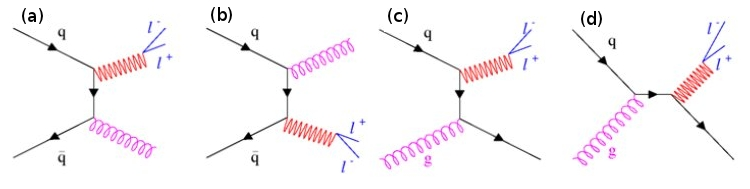
\includegraphics[width=5.00in]{figures/DY}
	\caption{The Drell-Yan process has a large range of higher-order QCD corrections that need to be accounted for. 
		(A) and (B) are high order $q\bar{q}$ annihilations, and (C) and (D) are gluon "Compton scattering" terms.}
	\label{fig:nlo-dy}
\end{figure}

Now the question is: what can the Drell-Yan process tell us that the well-exercised DIS scattering cannot? The core answer to that is that DIS is not intrinsically sensitive to flavor, whereas DY is. However, to answer the question fully, we must discuss the distribution of quarks in a nucleon.  

Let's say that we have two hadrons A and B colliding; a parton of type \emph{a} ($u, d, s, g$, etc.) comes from A and carries with it a fraction of A's momentum ($x_A$).  The same goes for hadron B; a parton of type \emph{b} comes from B and carries momentum fraction $x_B$. Now, the probability of finding the discussed parton from A is given by $f_{a/A}(x_A)dx_A$. Likewise, the probability of finding the discussed parton from B is $f_{b/B}(x_B)dx_B$.  

These \emph{structure functions}, $f_{a/A}(x)$ are called the \emph{parton distribution functions} (PDF's), and they have been the focus of a great deal of experiments over the years by several collaborations. Due to the complex nature of lattice QCD, these PDF's are determined empirically, with only a few rules based in theory. It is important to note that there is normally a $Q^2$ dependence of these PDF's. At high enough $Q^2$, as it is in the case of our experiment, the PDF's no longer scale with $Q^2$ \cite{Seely:2009gt}.  That is, for a given \emph{x}, the PDF is independent of $Q^2$.

An important metric to observe is the probability that a parton \emph{a} carries a momentum fraction $x_A$ in its hadron $A$.  This can be represented by the following expression: $x_A f_{a/A}(x_A)dx_A$. For Drell-Yan interactions in the study proposed here, we are interested in the momentum distribution amongst the quarks in the proton.  The CTEQ collaboration has collected data from many experiments, yielding the model represented in Figure \ref{fig:pdf} \cite{Pumplin:2002vw}.

\begin{figure}
	\centering
	\subfloat[][The parton distribution function describing the momentum carried by different types of quark in the proton.]{%
		\label{fig:pdf}%
		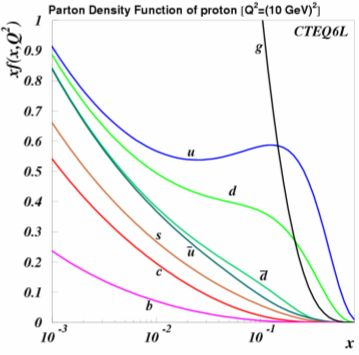
\includegraphics[width=0.40\linewidth]{figures/parton-dist.jpg}}%
	\hspace{8pt}%
	\subfloat[][The ratio of cross sections (per nucleon) as a function of the target's fractional momentum, $x_2$.  The EMC Effect region, $0.3<x_2<0.6$ is the phenomenon discussed here.]{%
		\label{fig:emc}%
		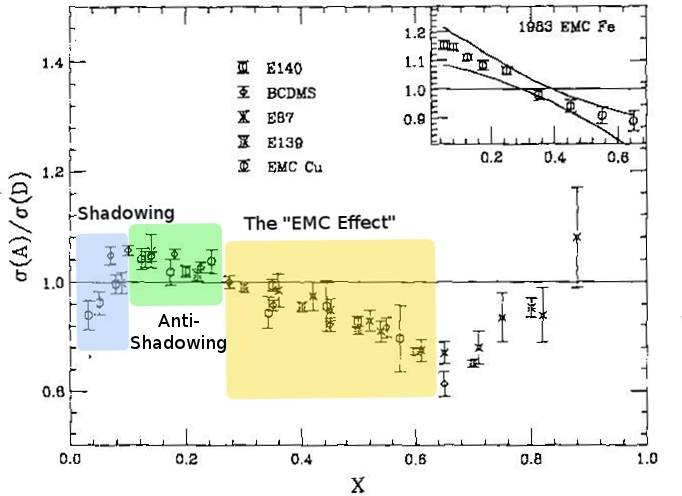
\includegraphics[width=0.53\linewidth]{figures/EMC_EMC.jpeg}}
	\caption{The proton's momentum distribution and the EMC Effect, with key regions highlighted.}
	\label{fig:pdf_emc}
\end{figure}

Looking to Figure \ref{fig:pdf} we see that at $x>0.1$, $u$ and $d$ quarks dominate $\bar{u}$ and $\bar{d}$ quarks.  This is key, because this means that, for SeaQuest where we have high $x_1$ and lower $x_2$, the Drell-Yan process is probabilistically dominated by a quark from the beam annihilating with an antiquark from the target. All antiquarks that exist in the target nucleons must come from what are called the \emph{sea quarks}, or the virtual $q\bar{q}$ pairs that pop in and out of existence amongst the gluons and valence quarks. 

As we will discuss in the next section, partons in a bound nucleon behave differently than partons in a free nucleon. By studying Drell-Yan in nuclear targets, we can investigate the degree to which this modification is the result of a modification to the quark sea.

\subsection{The Drell-Yan Cross-Section}

\subsection{Drell-Yan Kinematics}

\section{The EMC Effect}

The European Muon Collaboration, in 1983, measured the DIS cross section per nucleon ratios of $Fe$ to $D$ over a large kinematic range.  The result, as seen in the top right of Figure \ref{fig:emc} came as quite a surprise.  It was revealed that the structure function of a nucleon bound in a nucleus differs fundamentally from that of a free nucleon  \cite{Aubert:1983xm}.  This difference was not a simple or small effect either; the cross section per nucleon of a nucleus showed to be smaller than that of deuterium at very low $x_2$, greater than deuterium at $0.1<x_2<0.2$, and then steadily less than deuterium for $0.2<x_2<0.6$. 

This complex, unexplained behavior opened up a new field of research and theoretical work. Following suit, the different aspects of this nuclear modification garnered some common nicknames.  The region where $x_2<0.1$ became known as \emph{"Nuclear Shadowing"}, the transition region of $0.1<x_2<0.2$ is known as \emph{"Anti-shadowing"}, and the linear decline in the ratio of cross sections between $0.2<x_2<0.6$ is generally referred to as the \emph{"EMC Effect"} \cite{Geesaman:1995yd}.

The phenomenon was simple -- DIS off of a bound nucleon was not the same as off of a free nucleon -- but hundreds of theoretical papers were written attempting to explain it away, from multiquark ($6q$) clusters to the exchange of virtual pions in the nucleus. Some have joked that EMC should stand for \emph{"Every Model is Cool"}. The focus of recent work (and this paper) is on the "EMC Effect" region, characterized by the distinctly linear downward slope.

Recent experiments at Hall C at JLab and SLAC suggest the following regarding the EMC Effect \cite{Seely:2009gt}:
\begin{itemize}
	\item
	It is $Q^2$-independent
	\item
	It's x-dependent shape is universal (across various nuclei)
	\item
	The magnitude (slope) of the effect varies with A
	\item
	It thereby might be related to nuclear density
\end{itemize}

In parallel to this effort, many researchers were working on high-momentum nucleons and short range correlations (SRC's), neither aware yet of their common ground.